\documentclass[a4paper]{article}
\usepackage{fancyhdr}
\usepackage[usenames, dvipsnames]{xcolor}
\usepackage{graphicx,hyperref,amsmath,float,subfigure,soul}
\usepackage[top=3cm,bottom=3cm,left=3cm,right=3cm]{geometry}
\hypersetup{
	colorlinks,
	citecolor=black,
	filecolor=black,
	linkcolor=black,
	urlcolor=black
}
\newcommand{\HRule}{\rule{\linewidth}{0.5mm}}
\pagestyle{fancy}
\lfoot{\small \color{gray}Tom Peerdeman - 10266186}
\cfoot{\thepage}
\rfoot{\small \color{gray}Ren\'e Aparicio Sa\'ez - 10214054}
\lhead{\small \color{gray} OMP}
\begin{document}
	\begin{titlepage}
	\begin{center}
		\textsc{\Large Concurrency \& Parallel Programming}\\[0.5cm]
		\HRule \\[0,4cm]
		\textsc{\huge \bfseries OMP}
		\HRule \\[8cm]
		\begin{minipage}{0.4\textwidth}
			\begin{flushleft}\large
				\emph{Auteurs: Tom Peerdeman \& Ren\'e Aparicio Saez}\\
			\end{flushleft}
		\end{minipage}
		\begin{minipage}{0.4\textwidth}
			\begin{flushright}\large
			\emph{Datum: 19-11-2012\\\hspace{1cm}}\\
			\end{flushright}
		\end{minipage}
	\end{center}
	\end{titlepage}

  \section{Assignment 1.1 - Wave simulation}
  \subsection{Table with results}
    Tests on DAS4 are run for i = 1.000.000 and t = 1.000.
    The amount of omp threads used to generate the waves is increased
    to measure the difference in speed for the program.
    Each amount of threads is run 12 times. 
    The highest value and the lowest value are disregarded. 
    The remaining data is used to plot a graph.
    These tests are done without considering scheduling,
    this is done later in the report.\\\\
    \begin{tabular}{| c | c | c | c | c | c | c | c |}
      \hline
      \multicolumn{4}{|c}{i = 1,000,000} & \multicolumn{4}{c|}{t = 1,000}\\
      \hline
\st{3.1211} & 1.43211 & 1.26944 & 0.939188 & 0.851557 & 0.623673 & 0.718125 & 0.677228\\
      \hline
3.04543 & 1.42686 & 1.29452 & 0.813184 & 0.873015 & 0.654943 & 0.756256 & \st{0.587986}\\
      \hline
\st{3.02998} & \st{1.40477} & 1.33823 & 0.813059 & 0.848276 & \st{0.593785} & 0.740096 & \st{0.694887}\\
      \hline
3.0661 & 1.4104 & 1.45341 & 0.772554 & 0.878858 & 0.670092 & 0.720322 & 0.631909\\
      \hline
3.06365 & 1.41057 & \st{1.68411} & 0.814582 & \st{0.988416} & 0.630324 & 0.736533 & 0.664366\\
      \hline
3.08719 & 1.42461 & 1.30602 & \st{0.939831} & \st{0.828244} & 0.621332 & \st{0.716592} & 0.663344\\
      \hline
3.08742 & \st{2.20822} & 1.27907 & 0.802773 & 0.91554 & 0.628798 & 0.816578 & 0.622237\\
      \hline
3.04847 & 1.41933 & 1.30155 & 0.837648 & 0.854704 & 0.617878 & 0.833466 & 0.601991\\
      \hline
3.06515 & 1.44256 & 1.45228 & 0.913682 & 0.839151 & \st{0.708951} & \st{0.845428} & 0.677083\\
      \hline
3.04467 & 1.42778 & 1.29303 & \st{0.771725} & 0.845102 & 0.66214 & 0.731911 & 0.615128\\
      \hline
3.03383 & 1.44278 & 1.32129 & 0.825917 & 0.868847 & 0.666777 & 0.736191 & 0.592873\\
      \hline
3.07641 & 1.43763 & \st{1.26484} & 0.778603 & 0.89026 & 0.571218 & 0.73283 & 0.659633\\
      \hline
      \multicolumn{8}{|l|}{Average of the remaining 10:}\\
      \hline
      3.061832 & 1.424268 & 1.330884 & 0.8311174 & 0.8664933 & 0.6306423 & 0.7523437 & 0.6399728\\
      \hline
    \end{tabular}
    \begin{center}
      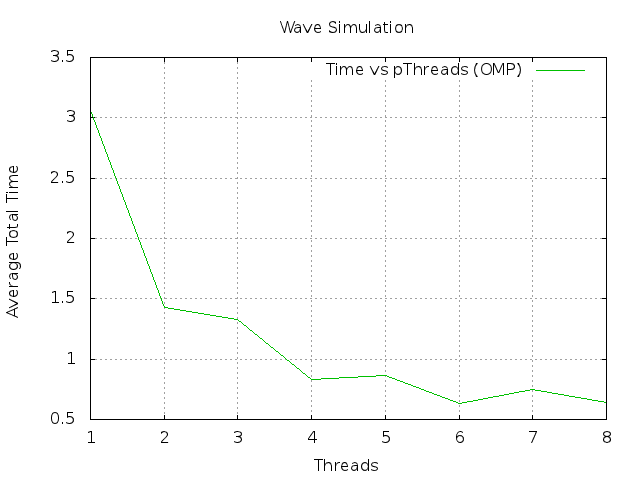
\includegraphics[width=0.9\textwidth]{speedplotsolo.png}
    \end{center}
    Apparantly the performance is better if an even number of threads is used.
  \newpage
  \subsection{Comparison to normal pThreads}
    When comparing the results, it becomes clear that OMP is faster then the usual pThread parallelisation method. The tests where done with normal scheduling\\
    \begin{tabular}{| l | c | c | c | c | c | c | c | c |}
      \hline
      \multicolumn{9}{|l|}{Average of 10 runs:}\\
      \hline
      pThreads & 3.788914 & 1.701978 & 1.713576 & 0.9564147 & 1.173655 & 0.7479494 & 0.89525656 & 0.6777506\\
      \hline
      OMP & 3.061832 & 1.424268 & 1.330884 & 0.8311174 & 0.8664933 & 0.6306423 & 0.7523437 & 0.6399728\\
      \hline
    \end{tabular}
    \begin{center}
      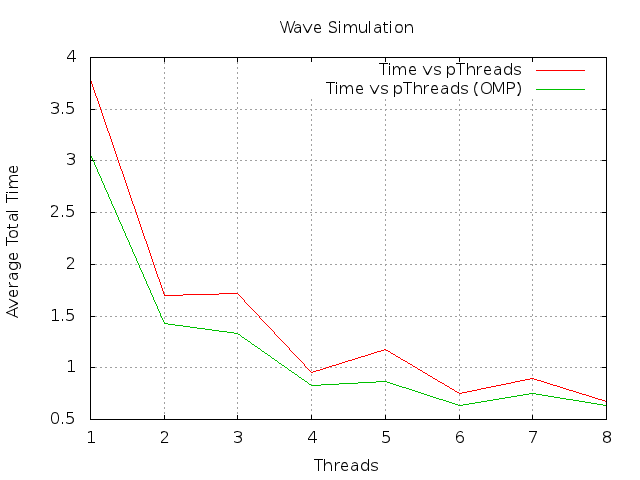
\includegraphics[width=0.9\textwidth]{speedplot.png}
    \end{center}
    
\end{document}
